\documentclass[10pt]{article}
\usepackage[a4paper, margin=.9in]{geometry}
% \usepackage{xeCJK}
% \setCJKmainfont{Microsoft YaHei} 
\newcommand{\DOUBLECOL}{}	% turns this on for double column
\newlength{\subfigureheight}
\newlength{\figurewidth}
\ifdefined\DOUBLECOL
\setlength{\subfigureheight}{2.45in}
\setlength{\figurewidth}{3.5in}
\else
\setlength{\subfigureheight}{2.35in}
\setlength{\figurewidth}{6.5in}
\fi
\usepackage{amsfonts,amsmath,amssymb,bm,cancel,color,comment,epsfig,enumerate,empheq,floatrow,hyperref,mathdots,mathrsfs}
\usepackage{placeins}%\usepackage{algorithmic}
\usepackage[vlined,ruled,linesnumbered]{algorithm2e}
\SetKwInput{KwInput}{Input}                % Set the Input
\SetKwInput{KwOutput}{Output}              % set the Output
\SetKwRepeat{Do}{do}{until}%
\usepackage{graphicx}
%\usepackage{amsthm}
\usepackage[super]{nth}
\usepackage[noadjust]{cite}
\usepackage{subcaption}
\usepackage{tabularx}
\usepackage{tabularray}		% make thing horizontal lines in tabular
\UseTblrLibrary{booktabs}	% make thing horizontal lines in tabular

\usepackage{listings}
\usepackage{xcolor}

% --- MATLAB code style ---
\lstdefinelanguage{Matlab}{
  morekeywords={break,case,catch,continue,else,elseif,end,for,function,
    global,if,otherwise,persistent,return,switch,try,while},
  sensitive=true,
  morecomment=[l]\%,
  morestring=[m]',
}
\lstset{
  language=Matlab,
  basicstyle=\ttfamily\small,
  keywordstyle=\color{blue}\bfseries,
  commentstyle=\color{gray},
  stringstyle=\color{red!70!black},
  numbers=left,
  numberstyle=\tiny,
  stepnumber=1,
  numbersep=5pt,
  frame=single,
  breaklines=true,
  showstringspaces=false,
  columns=fullflexible
}


% --- TikZ setup ---
\usepackage{tikz}
\usetikzlibrary{positioning,shapes,arrows.meta,calc}
\usetikzlibrary{decorations.pathreplacing}

% \tikzstyle{block} = [rectangle, rounded corners, minimum width=3cm, minimum height=1cm,
%                      text centered, draw=black, fill=blue!10]
% \tikzstyle{arrow} = [thick,->,>=stealth]

\tikzset{
  >={Latex[length=3mm]},
  block/.style={draw, thick, rectangle, minimum width=2.8cm, minimum height=1.2cm, align=center},
  filter/.style={draw, thick, trapezium, trapezium left angle=70, trapezium right angle=110,
                 minimum width=3.0cm, minimum height=1.2cm, align=center},
  mixer/.style={circle, draw, thick, minimum size=8mm, inner sep=0pt,
                path picture={
                  \draw[]
                    (-2.4mm,-2.4mm)--(2.4mm,2.4mm)
                    (-2.4mm,2.4mm)--(2.4mm,-2.4mm);
                }},
  conn/.style={thick, -{Latex}}
}

% \graphicspath{{eps/}}

\hypersetup{
	colorlinks=true,
	linkcolor=red,
	citecolor=green,
	filecolor=magenta,
	urlcolor=blue
}


\newenvironment{Ualgorithm}[1][htpb]{\def\@algocf@post@ruled{\kern\interspacealgoruled\hrule  height\algoheightrule\kern3pt\relax}%
\def\@algocf@capt@ruled{under}
\begin{algorithm}[#1]}
{\end{algorithm}}

\setcounter{MaxMatrixCols}{30}
\DeclareSymbolFont{grb}{OML}{cmm}{b}{it}
\DeclareMathSymbol{\zetab}{\mathord}{grb}{"10}
\DeclareMathSymbol{\etab}{\mathord}{grb}{"11}
\DeclareMathSymbol{\thetab}{\mathord}{grb}{"12}
\DeclareMathSymbol{\kappab}{\mathord}{grb}{"14}
\DeclareMathSymbol{\lambdab}{\mathord}{grb}{"15}
\DeclareMathSymbol{\mub}{\mathord}{grb}{"16}
\DeclareMathSymbol{\nub}{\mathord}{grb}{"17}
\DeclareMathSymbol{\rhob}{\mathord}{grb}{"1A}
\DeclareMathSymbol{\sigmab}{\mathord}{grb}{"1B}
\DeclareMathSymbol{\taub}{\mathord}{grb}{"1C}
\DeclareMathSymbol{\phib}{\mathord}{grb}{"1E}
\DeclareMathSymbol{\psib}{\mathord}{grb}{"20}
\DeclareMathSymbol{\omegab}{\mathord}{grb}{"21}
\DeclareMathSymbol{\epsilonb}{\mathord}{grb}{"22}
\DeclareMathSymbol{\varphib}{\mathord}{grb}{"27}
\input{Symbol_Shortcut.tex}

\newtheorem{theorem}{\bf Theorem}		% by Victor
\newtheorem{corollary}{\bf Corollary}	% by Victor
\newtheorem{definition}{\bf Definition}	% by Victor

%\centerfigcaptionstrue

%\pagestyle{empty}

\makeatletter
\def\ifundefined{\@ifundefined}
\makeatother

\setlength{\parskip}{0ex}

% generating the double accent on o, i.e. \fH{o}, e.g. Erdos Renyi 
\newcommand\fH[1]{\sbox0{#1}\dimen0=\ht0 \advance\dimen0 -1ex
  \sbox2{\'{}}\sbox2{\raise\dimen0\box2}%
  {\ooalign{\hidewidth\kern.1em\copy2\kern-.5\wd2\box2\hidewidth\cr\box0\crcr}}}

\title{\vspace{-0.2em} \huge LAB1 Report}

% \ifdefined \BLIND
\author{Pin-Jing, Li (111511015 \it{ouo.ee11@nycu.edu.tw})\\ 
Jing-Kai, Huang\\ 
Duan-Kai, Wu}





% \markboth{IEEE Trans. on Communications}{Model-Driven Based MIMO Channel Estimator}
\begin{document}
\maketitle


% \begin{IEEEkeywords}
% \end{IEEEkeywords}
In lab 1 We explored the basic configuration of $\mathrm{e}^2$ studio, ultrasound module and the basic signal processing flow of the wireless transmitted signal.



%%%%%%%%%%%%%%%%%%%%%%%%%%%%%%%%%%%%%%%%%%%%%%%%%%%%%%%%%%%%%%%%%%
\section{Hardware configuration}
%%%%%%%%%%%%%%%%%%%%%%%%%%%%%%%%%%%%%%%%%%%%%%%%%%%%%%%%%%%%%%%%%%


%%%%%%%%%%%%%%%%%%%%%%%%%%%%%%%%%%%%%%%%%%%%%%%%%%%%%%%%%%%%%%%%%%
\section{Error Source Analysis}
%%%%%%%%%%%%%%%%%%%%%%%%%%%%%%%%%%%%%%%%%%%%%%%%%%%%%%%%%%%%%%%%%%


We inspect the relative distance and try to determine the model of the error.

\begin{table}[h!]
\centering
\caption{Relative Distance Comparison (Measured vs. Theoretical)}
\begin{tabular}{|c|c|c|c|c|c|c|}
\hline
Pair (cm) & $n^*_{\mathrm{theory}}$ & $n_{\mathrm{meas}}$ & 
$\Delta n^*_{\mathrm{theory}}$ & $\Delta n_{\mathrm{meas}}$ &
$\frac{\Delta n_{\mathrm{meas}}}{\Delta n^*_{\mathrm{theory}}}$ & 
Relative Error (\%) \\
\hline
20→40 & 184.97$\rightarrow$369.94 & 231$\rightarrow$412 & 184.97 & 181 & 0.979 & -2.1 \\
40→60 & 369.94$\rightarrow$554.91 & 412$\rightarrow$598 & 184.97 & 186 & 1.006 & +0.6 \\
60→80 & 554.91$\rightarrow$739.88 & 598$\rightarrow$773 & 184.97 & 175 & 0.946 & -5.4 \\
80→100 & 739.88$\rightarrow$924.86 & 773$\rightarrow$953 & 184.97 & 180 & 0.973 & -2.7 \\
\hline
\end{tabular}
\end{table}

We retrieve back $n_\mathrm{meas}$ by aligning the starting sample by the maximum Tx data 

We plot out the 
\begin{figure}[!h]
	\centering 
	\subcaptionbox{Measured Peak and the theoretical sample (T=25)
		\label{fig:sample_meas_theo}} {
		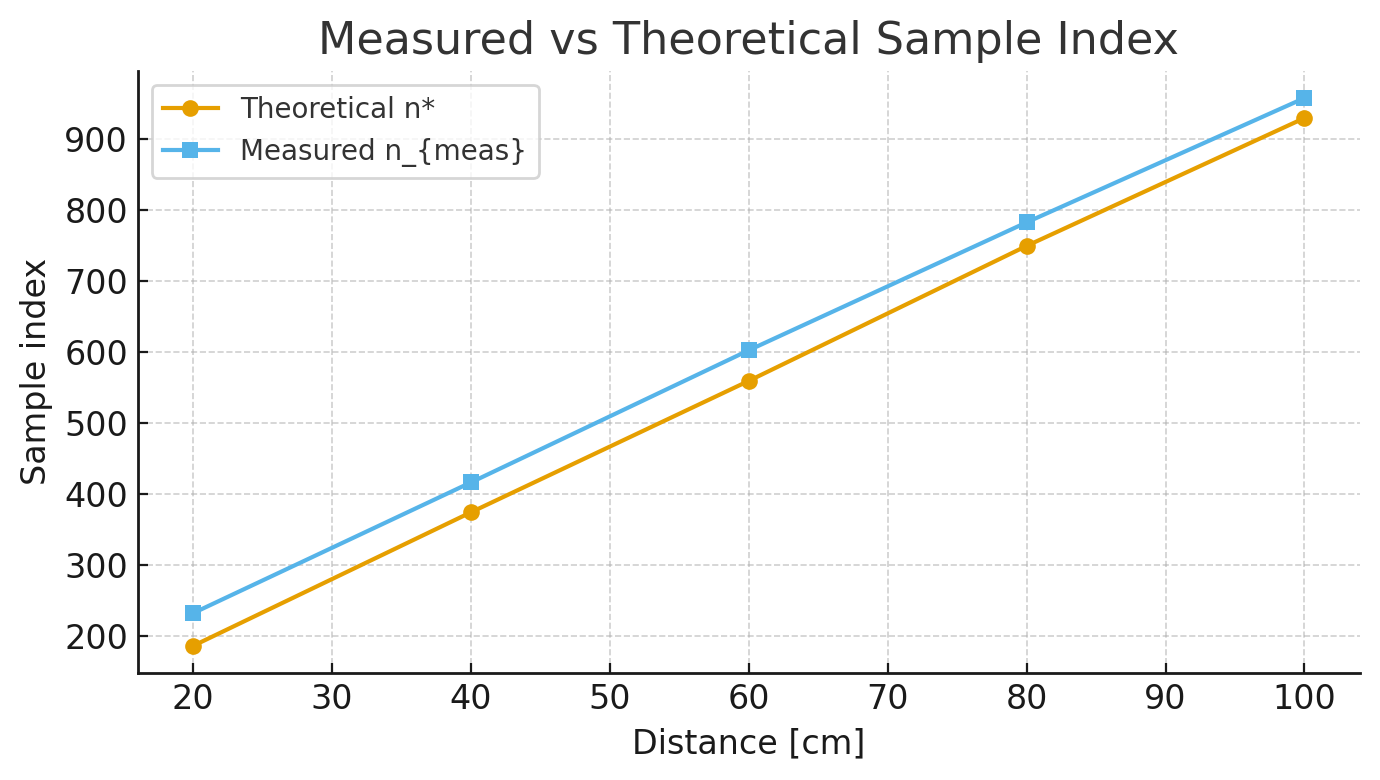
\includegraphics[width = .45\columnwidth]{fig/distance_vs_sample_theo_meas.png}	
	}
	\subcaptionbox{Error vs. distance 
		\label{fig:error_vs_dist}} {
		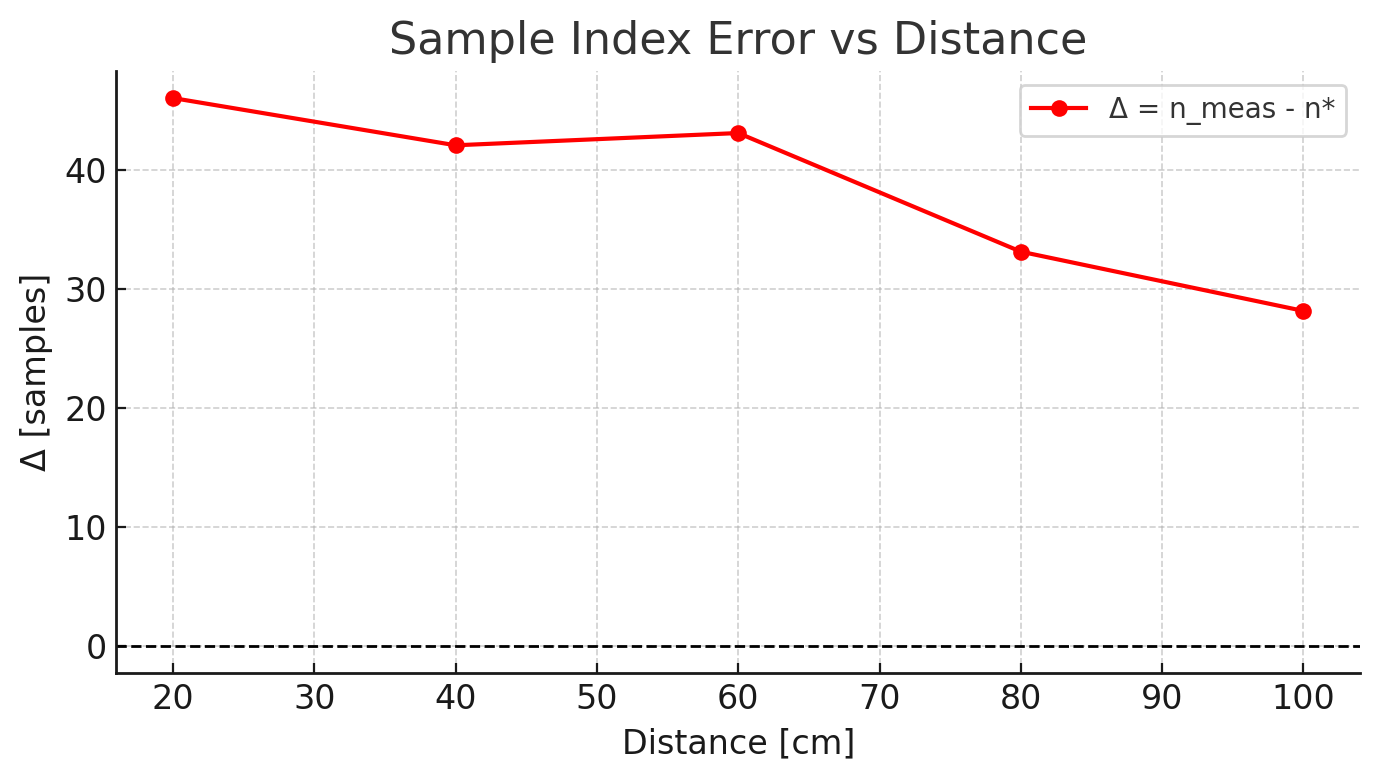
\includegraphics[width = .45\columnwidth]{fig/distance_vs_delta.png}
	}
	\caption{Comparing robust and non-robust design for linear precoder}
\label{fig:robust_lin}
\end{figure}


$$
\Delta = a + b n_\mathrm{meas}
$$

With linear regression we found $a \simeq 53.14, b \simeq -0.02469$, and we therefore perform the correction on the measurements


\begin{table}[h!]
\centering
\caption{Corrected Sample Index and Residual Distance Error (Linear Model)}
\begin{tabular}{c|c|c|c|c}
\hline
True Distance (cm) & $n_{\mathrm{meas}}$ & $\hat{n}$ (Corrected) & $n^{*}$ (Theory) & Error After Correction (cm) \\
\hline
20  & 231 & 183.56 & 184.97 & $-0.15$ \\
40  & 412 & 369.04 & 369.94 & $-0.10$ \\
60  & 598 & 559.39 & 554.91 & $+0.48$ \\
80  & 773 & 738.65 & 739.88 & $-0.13$ \\
100 & 953 & 922.23 & 924.86 & $-0.28$ \\
\hline
\end{tabular}
\end{table}

% \begin{figure}[!h]
% 	\centering 
% 		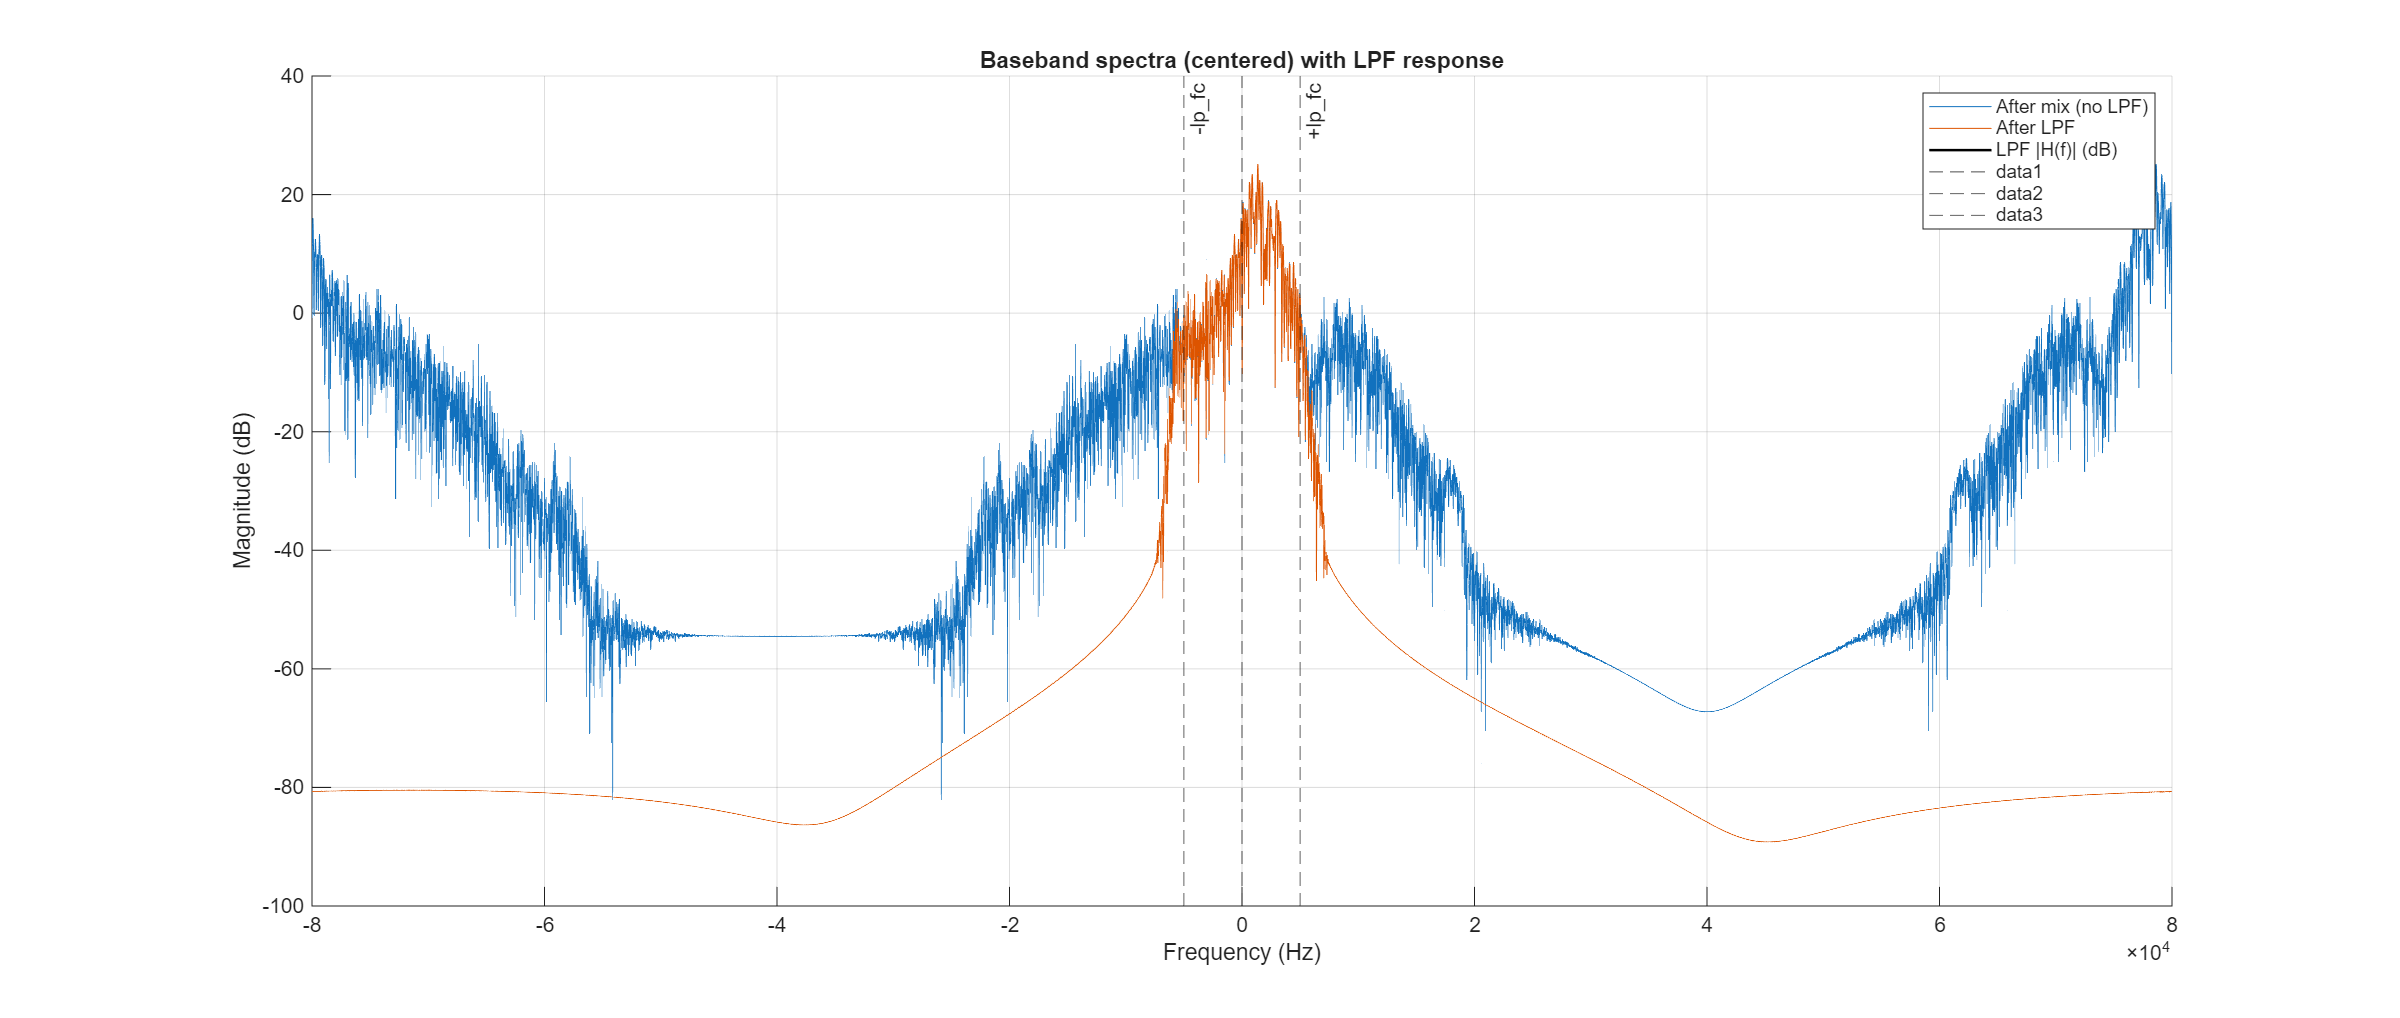
\includegraphics[width = .75\columnwidth]{fig/100_fdomain_bb_lp.png}	
% 	\caption{}
% \label{fig:bb_lp}
% \end{figure}


%%%%%%%%%%%%%%%%%%%%%%%%%%%%%%%%%%%%%%%%%%%%%%%%%%%%%%%%%%%%%%%%%%
\section{Signal Processing}
%%%%%%%%%%%%%%%%%%%%%%%%%%%%%%%%%%%%%%%%%%%%%%%%%%%%%%%%%%%%%%%%%%
\begin{figure}[h!]
\centering
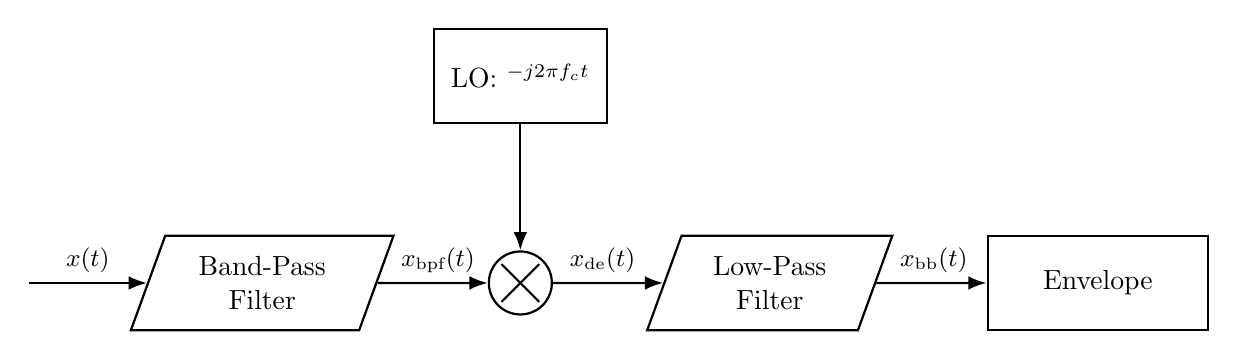
\begin{tikzpicture}[node distance=2.0cm and 1.4cm]

% Nodes (main chain)
% \node (x)    [block, draw=none] {};
\node (bpf)  [filter] {Band-Pass\\Filter};
\node (mix)  [mixer,  right=of bpf] {};
\node (lpf)  [filter, right=of mix] {Low-Pass\\Filter};
\node (env)  [block,  right=of lpf] {Envelope};

% LO branch (for demodulator)
\node (lo)   [block, above=1.6cm of mix, minimum width=2.2cm] {LO: $\e^{-j2\pi f_c t}$};

% Connections
% \draw[conn] (x) -- (bpf);
\draw[conn] ([xshift=-1.5cm]bpf.west) -- (bpf.west);
\draw[conn] (bpf) -- (mix);
\draw[conn] (mix) -- (lpf);
\draw[conn] (lpf) -- (env);
\draw[conn] (lo)  -- (mix);

% Optional labels on interconnects
\node[above, font=\small] at ($(bpf.west)!0.5!([xshift=-1.5cm]bpf.west)$) {$x(t)$};
\node[above right,  font=\small] at ($(bpf)!0.5!(mix)$) {$x_{\text{bpf}}(t)$};
\node[above left,  font=\small] at ($(mix)!0.5!(lpf)$) {$x_{\text{de}}(t)$};
\node[above, font=\small] at ($(lpf)!0.5!(env)$) {$x_\text{bb}(t)$};

\end{tikzpicture}
\caption{block diagram: signal $\rightarrow$ BPF $\rightarrow$ demod (mixer) $\rightarrow$ LPF $\rightarrow$ envelope.}
\label{fig:sp-chain}
\end{figure}

some discussion below:
\begin{itemize}
	\item \textbf{Correct "Detection" threshold. } The physically correct measure of the time of flight (TOF) would be the \textit{wavefront} of the received signal.
\end{itemize}

\begin{figure}[!h]
	\centering 
		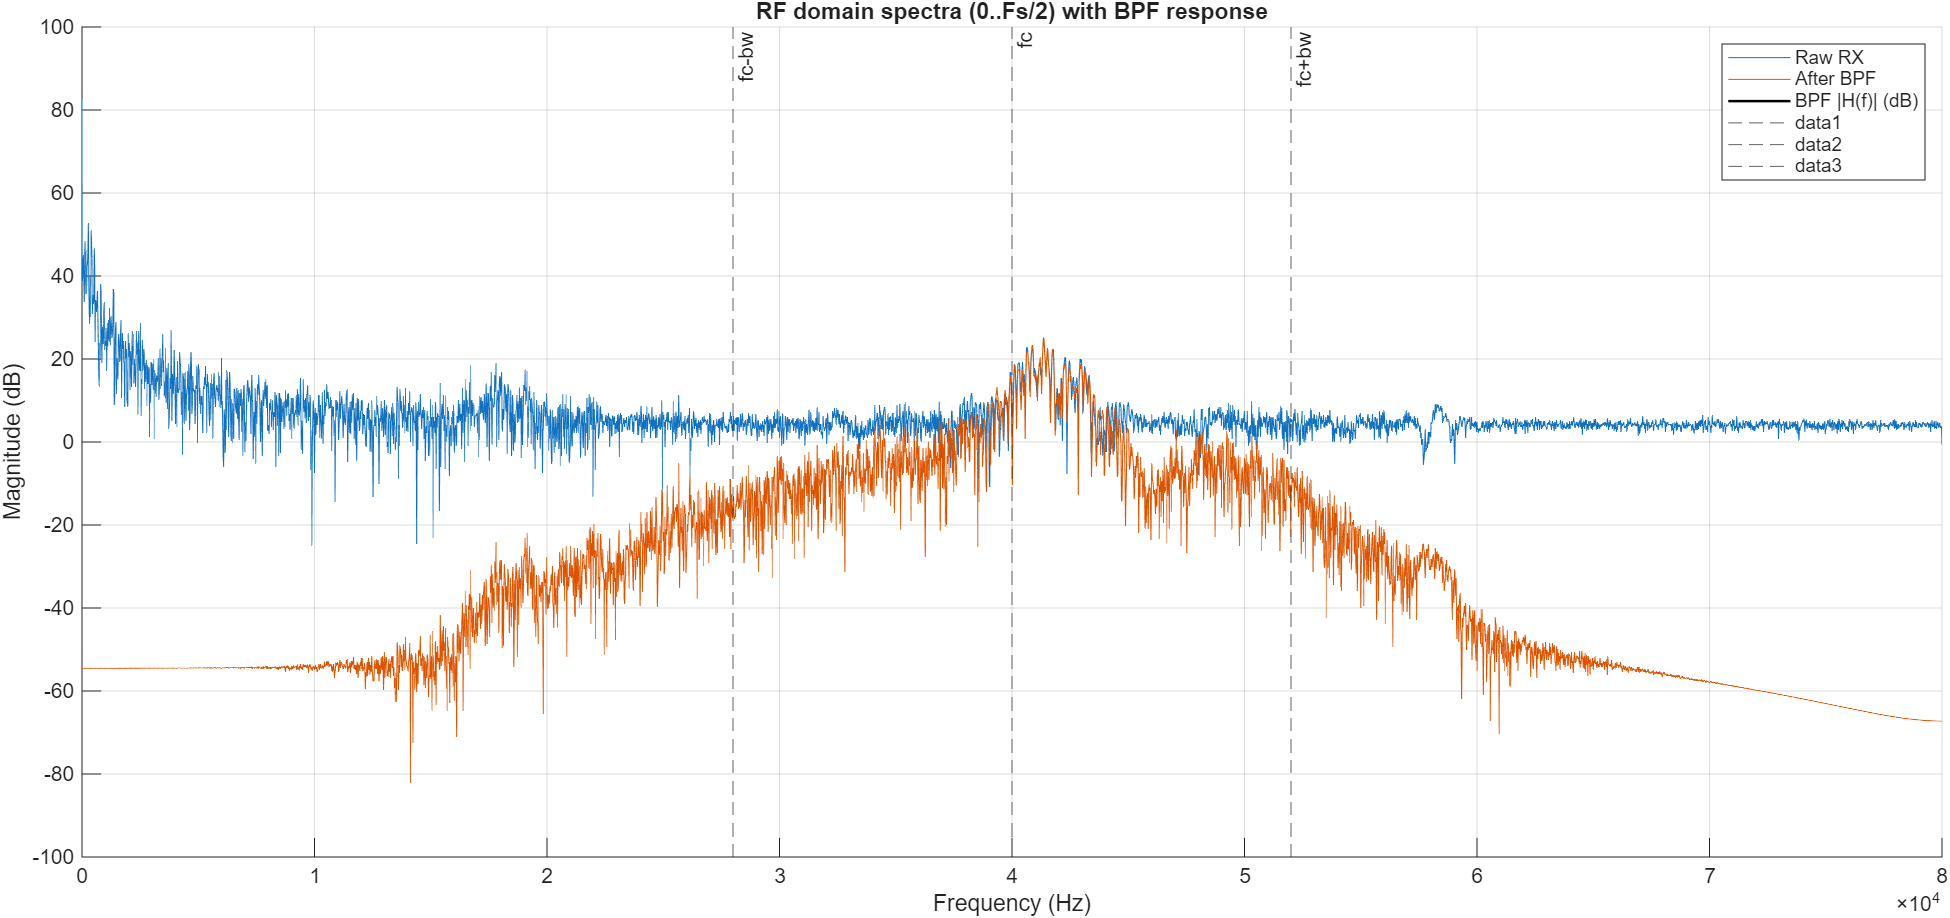
\includegraphics[width = .75\columnwidth]{fig/100_fdomain_bpf.png}	
	\caption{bpf}
\label{fig:bpf}
\end{figure}

\subsection*{Bandpass Filtering}

Given the sampled received signal $x(t)$, we first apply a bandpass filter to isolate the signal components near the carrier frequency. The bandpass-filtered signal is

\begin{equation}
x_{\mathrm{bpf}}(t) = x(t) * h_{\mathrm{bpf}}(t)
\end{equation}

where $*$ denotes convolution and $h_{\mathrm{bpf}}(t)$ is the impulse response of the bandpass filter.  

\paragraph{Filter Design.}
We choose a $6^{\text{th}}$-order IIR Butterworth bandpass filter with half-power frequencies
\[
f_{\mathrm{bp},1} = f_c - 2f_w, \qquad
f_{\mathrm{bp},2} = f_c + 2f_w,
\]
where the carrier frequency $f_c = 40~\mathrm{kHz}$ and the signal bandwidth is
\[
f_w = \frac{1}{T_{\mathrm{burst}}} \approx 5~\mathrm{kHz}.
\]

To ensure the filter design remains within valid frequency bounds, we compute:
\[
\begin{aligned}
\texttt{bp\_bw} &= \max\!\bigl(2f_w,\, 12~\mathrm{kHz}\bigr),\\[4pt]
\texttt{bp\_f1} &= \max\!\bigl(10,\, f_c - \texttt{bp\_bw}\bigr),\\[4pt]
\texttt{bp\_f2} &= \min\!\bigl(\tfrac{F_s}{2}-10,\, f_c + \texttt{bp\_bw}\bigr),
\end{aligned}
\]
where $F_s$ is the sampling frequency.

\paragraph{MATLAB Implementation.}
The filter is implemented and applied using MATLAB as follows:

\begin{lstlisting}
bp_bw = max(2*fw, 12e3);            % Bandwidth selection
bp_f1 = max(10, fc - bp_bw);        % Lower cutoff frequency
bp_f2 = min(Fs/2-10, fc + bp_bw);   % Upper cutoff frequency

dbp = designfilt('bandpassiir','FilterOrder',6, ...
    'HalfPowerFrequency1', bp_f1, ...
    'HalfPowerFrequency2', bp_f2, ...
    'SampleRate', Fs);

rx_bp = filtfilt(dbp, rx_dc);       % Zero-phase filtering
\end{lstlisting}

This produces the zero-phase bandpass-filtered signal $x_{\mathrm{bpf}}(t)$.


\subsection*{Demodulation}

After bandpass filtering, we demodulate the signal by multiplying it with a complex exponential at the carrier frequency $f_c$:

\begin{equation}
x_{\mathrm{de}}(t) = x_{\mathrm{bpf}}(t) \cdot e^{-j 2 \pi f_c t}
\end{equation}

In the frequency domain, this shifts the bandpass signal to baseband, centering its spectrum around $0$ Hz.


\begin{lstlisting}
w0 = 2*pi*fc/Fs;             % Normalized carrier frequency (rad/sample)
lo = exp(-1j*w0*n);          % Complex exponential for downconversion
bb = rx_bp .* lo;            % Complex baseband signal
\end{lstlisting}

\begin{figure}[!h]
	\centering 
		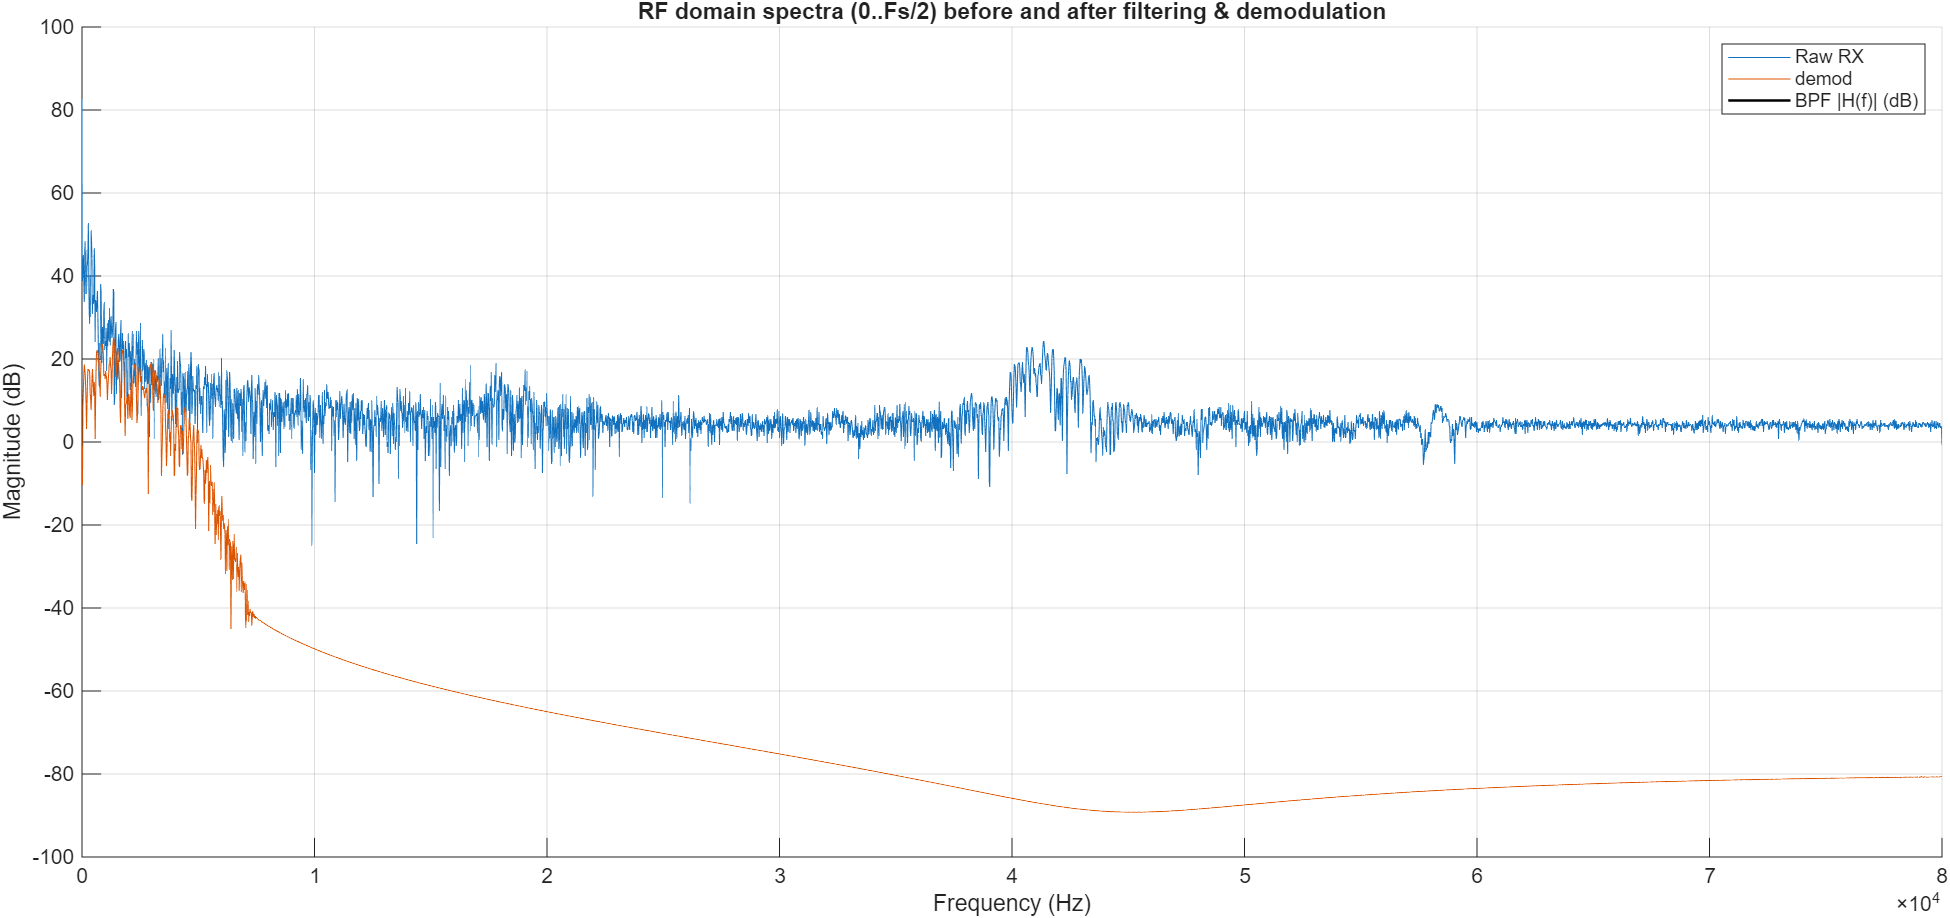
\includegraphics[width = .75\columnwidth]{fig/100_fdomain_demod.png}	
	\caption{demod}
\label{fig:demod}
\end{figure}

---

\subsection*{Low-Pass Filtering}

The downconverted signal still contains high-frequency components due to the product term.  
We pass $x_{\mathrm{de}}(t)$ through a low-pass filter to retain only the baseband component.

\paragraph{Filter Design.}

We use a FIR low-pass filter with passband edge at $f_{\mathrm{LP}} = f_{\mathrm{c}}$ and stopband starting at $1.6 f_{\mathrm{LP}}$:

\begin{lstlisting}
% FIR: passband up to lp_fc, stopband starts at 1.6*lp_fc
dlp = designfilt('lowpassfir', ...
    'PassbandFrequency', lp_fc, ...
    'StopbandFrequency', 1.6*lp_fc, ...
    'PassbandRipple', 0.1, ...          
    'StopbandAttenuation', 70, ...
    'SampleRate', Fs);

bb_f = filtfilt(dlp, real(bb)) + 1j*filtfilt(dlp, imag(bb));
\end{lstlisting}

This yields the complex baseband signal $x_{\mathrm{bb}}(t)$ with high-frequency components removed.

---

\subsection*{Envelope Detection}

Since the original signal is carried by $f_c$, it can be expressed as
\[
x(t) = A \cos(2\pi f_c t + \phi).
\]

After demodulation, we have
\[
\mathrm{Re}\{x_{\mathrm{de}}(t)\} = x(t)\cos(2\pi f_c t)
= \frac{A}{2} \bigl[\cos(\phi) + \cos(4 \pi f_c t + \phi)\bigr].
\]

Thus, the envelope amplitude is halved. We compensate for this loss by multiplying by $2$ when extracting the magnitude of the analytic signal:

\begin{lstlisting}
env = 2 * abs(bb_f);
\end{lstlisting}

This produces the envelope of the baseband signal, scaled back to its original amplitude.

\begin{figure}[!h]
	\centering 
		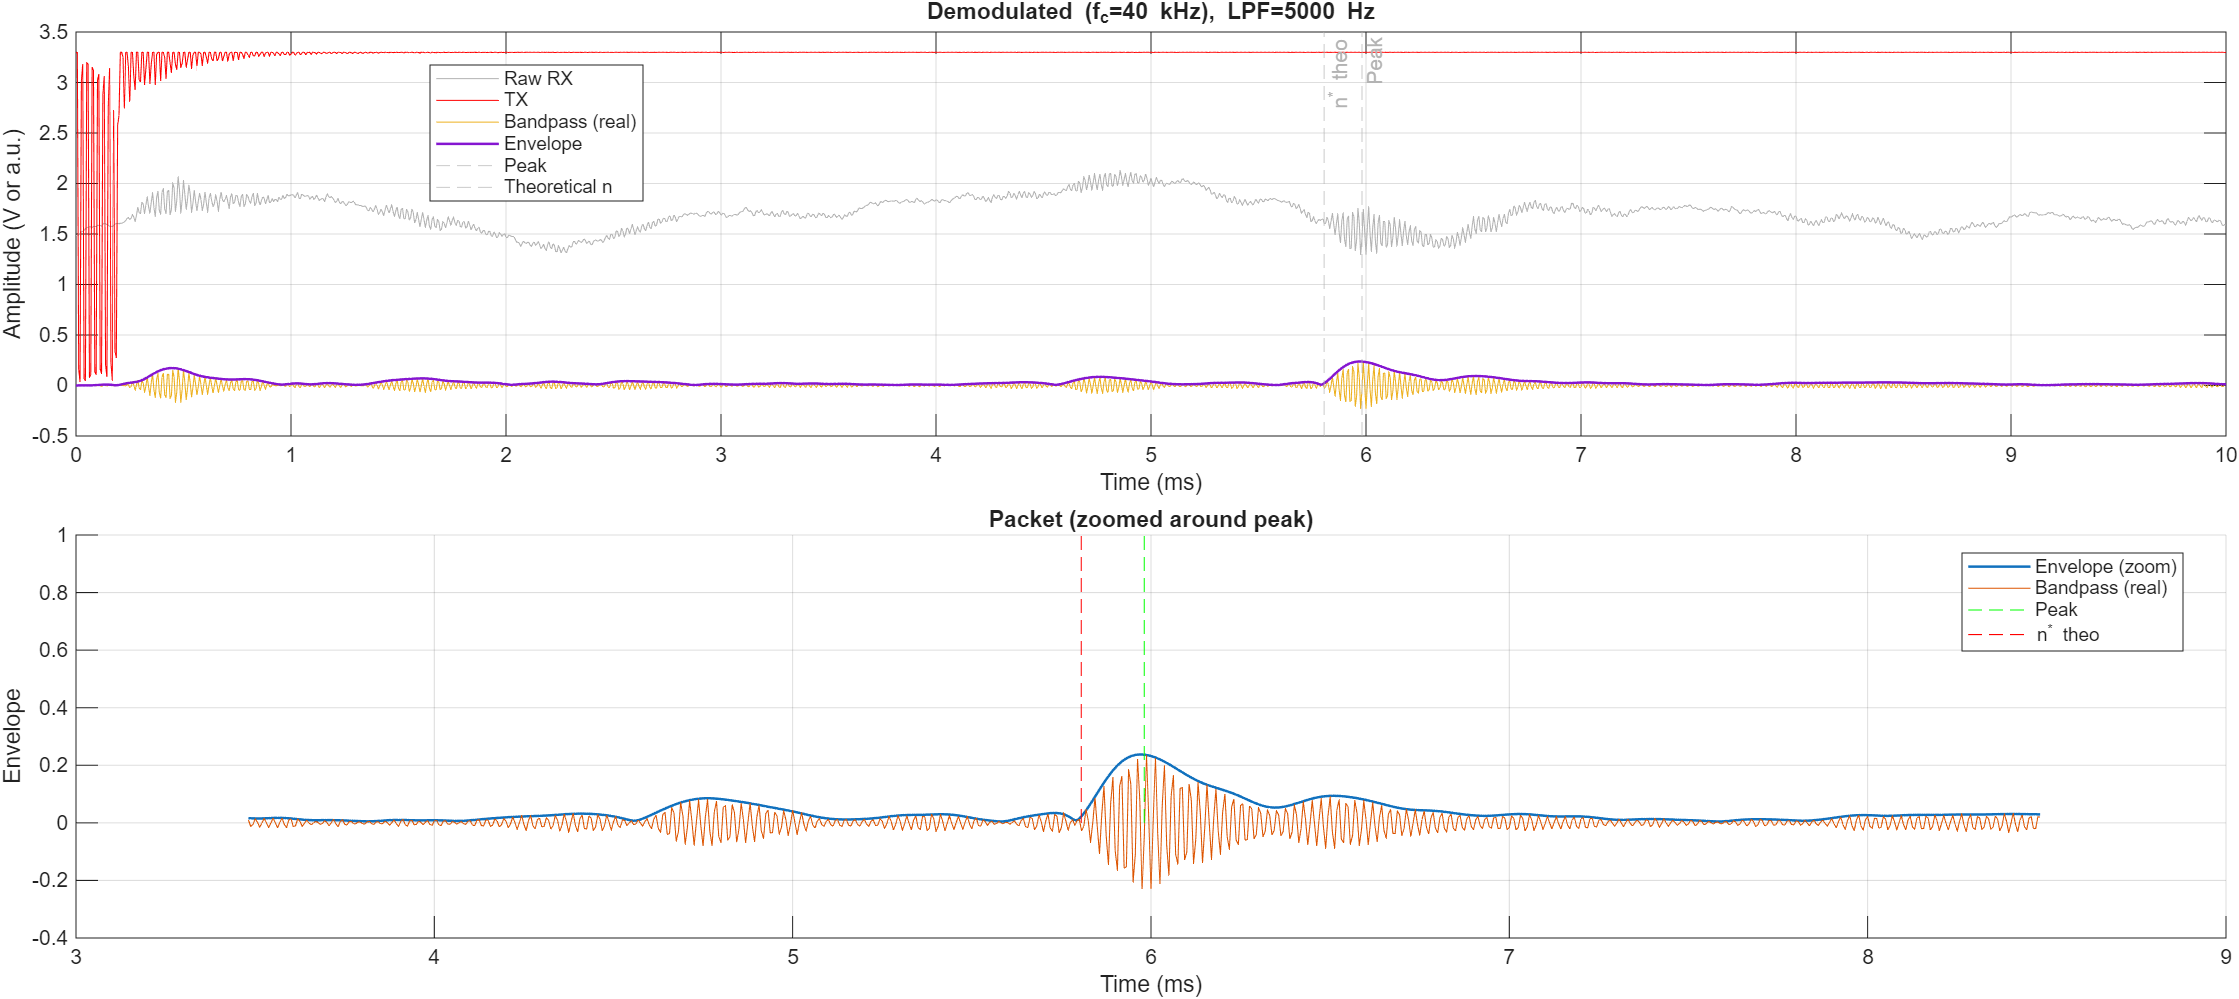
\includegraphics[width = .99\columnwidth]{fig/100_tdomain_raw_processed}	
	\caption{Time domain signal before and after filtering \& demodulation}
\label{fig:tdom_raw and processed}
\end{figure}




%%%%%%%%%%%%%%%%%%%%%%%%%%%%%%%%%%%%%%%%%%%%%%%%%%%%%%%%%%%%%%%%%%
\appendix{}


%%%%%%%%%%%%%%%%%%%%%%%%%%%%%%%%%%%%%%%%%%%%%%%%%%%%%%%%%%%%%%%%%%


\begin{thebibliography}{99}

\bibitem{chang2015semm}
C.-Y. Chang and C.C. Fung, ``Sparsity enhanced mismatch model for robust spatial intercell interference cancelation in heterogeneous networks,'' \emph{IEEE Trans. on Communications}, vol. 63(1), pp. 125-139, Jan. 2015.

\bibitem{ipr_realworld}
I. P. Roberts, Y. Zhang, T. Osman, and A. Alkhateeb, ``Real-world evaluation of full-duplex millimeter wave communication systems,'' \emph{IEEE Trans. Wireless Commun.}, early access, Mar. 2024.

\bibitem{ShenYu2018}
K.~Shen and W.~Yu, ``Fractional Programming for Communication Systems—Part I: Power Control and Beamforming,'' \textit{IEEE Transactions on Signal Processing}, vol.~66, no.~10, pp.~2616-2630, May 15, 2018, doi: 10.1109/TSP.2018.2812733.

\bibitem{ho2020denoising}
J.~Ho, A.~Jain, and P.~Abbeel, ``Denoising diffusion probabilistic models,'' 
\emph{Advances in Neural Information Processing Systems}, vol.~33, pp.~6840--6851, 2020.

\bibitem{o2017dl_phy_layer}
T.~O’Shea and J.~Hoydis, ``An introduction to deep learning for the physical layer,'' 
\emph{IEEE Transactions on Cognitive Communications and Networking}, vol.~3, no.~4, pp.~563--575, 2017.

\bibitem{Servetnyk2022} 
M.~Servetnyk and C.~C.~Fung, ``Distributed fronthaul-constrained joint transmission design and selection using augmented consensus-based dual decomposition,'' \textit{Journal of Communications and Networks}, vol.~24, no.~4, pp.~419--437, Aug.~2022, doi: \href{https://doi.org/10.23919/JCN.2022.000030}{10.23919/JCN.2022.000030}.

\end{thebibliography}
\end{document}




